\chapter{The Derivative}
\label{chp:derivative}			

\section{The \texttt{diff()} Command}

The \texttt{diff()} command is probably the most basic way of finding the derivative of an expression. The first parameter is the expression to be differentiated and the second parameter is the variable that the expression is to be differentiated with respect to.
\index{derivative!diff}
\index{mathematical functions!inverse tangent}
\index{mathematical functions!sine}
\index{subs}
\index{simplify}
\index{ditto operator}
\index{Pi}
\begin{maplegroup}
\begin{mapleinput}
\mapleinline{active}{1d}{diff(arctan(t), t);
}{}
\end{mapleinput}
\mapleresult
\begin{maplelatex}
\mapleinline{inert}{2d}{1/(t^2+1)}{\[\displaystyle  \frac{1}{{t}^{2}+1}\]}
\end{maplelatex}
\end{maplegroup}

If you have assigned a function, then make sure to use proper function notation inside the \texttt{diff()} command.

\begin{maplegroup}
\begin{mapleinput}
\mapleinline{active}{1d}{f(x) := sin(x);
}{}
\end{mapleinput}
\mapleresult
\begin{maplelatex}
\mapleinline{inert}{2d}{f := proc (x) options operator, arrow; sin(x) end proc}{\[\displaystyle f\, := \,x\mapsto \sin \left( x \right) \]}
\end{maplelatex}
\end{maplegroup}

\marginnote{Make sure that you are taking the derivative with respect to the desired variable.}
\begin{maplegroup}
\begin{mapleinput}
\mapleinline{active}{1d}{deriv1 := diff(f(x), x);
}{}
\end{mapleinput}
\mapleresult
\begin{maplelatex}
\mapleinline{inert}{2d}{deriv1 := cos(x)}{\[\displaystyle {\it deriv1}\, := \,\cos \left( x \right) \]}
\end{maplelatex}
\end{maplegroup}

\begin{maplegroup}
\begin{mapleinput}
\mapleinline{active}{1d}{slope := subs(x = Pi/2, deriv1); simplify(%);
}{}
\end{mapleinput}
\mapleresult
\begin{maplelatex}
\mapleinline{inert}{2d}{slope := cos((1/2)*Pi)}{\[\displaystyle {\it slope}\, := \,\cos \left( \pi/2 \right) \]}
\end{maplelatex}
\mapleresult
\begin{maplelatex}
\mapleinline{inert}{2d}{0.}{\[\displaystyle  0\]}
\end{maplelatex}
\end{maplegroup}

\subsection{Higher Derivatives using \texttt{diff()}}

Higher derivatives can be evaluated by applying the \texttt{diff()} command multiple times, by specifying the variable repetitively, or using the \$ notation, as shown below.
\index{derivative!diff!higher derivatives}
\begin{maplegroup}
\begin{mapleinput}
\mapleinline{active}{1d}{diff(arctan(t), t); diff(%,t); 
}{}
\end{mapleinput}
\mapleresult
\begin{maplelatex}
\mapleinline{inert}{2d}{1/(t^2+1)}{\[\displaystyle  \frac{1}{{t}^{2}+1}\]}
\end{maplelatex}
\mapleresult
\begin{maplelatex}
\mapleinline{inert}{2d}{-2*t/(t^2+1)^2}{\[\displaystyle -\,{\frac {2t}{ \left( {t}^{2}+1 \right) ^{2}}}\]}
\end{maplelatex}
\end{maplegroup}

\begin{maplegroup}
\begin{mapleinput}
\mapleinline{active}{1d}{diff(f(x), x, x);
}{}
\end{mapleinput}
\mapleresult
\begin{maplelatex}
\mapleinline{inert}{2d}{-sin(x)}{\[\displaystyle -\sin \left( x \right) \]}
\end{maplelatex}
\end{maplegroup}

\begin{marginfigure}
\centering
\includegraphics[scale=0.8]{tutorials/figures/palettediff.png}
\caption{You can also make use of quick shortcuts from the Calculus palette.}
\end{marginfigure}

\begin{maplegroup}
\begin{mapleinput}
\mapleinline{active}{1d}{diff(f(x), x$2);
}{}
\end{mapleinput}
\mapleresult
\begin{maplelatex}
\mapleinline{inert}{2d}{-sin(x)}{\[\displaystyle -\sin \left( x \right) \]}
\end{maplelatex}
\end{maplegroup}

\section{Using Function Notation}

If you have properly defined a function $f(x)$, you may also make use of the familiar $f'(x)$ notation used in class.
\index{derivative!prime notation}
\index{mathematical functions!sine}
\index{Pi}
\begin{maplegroup}
\begin{mapleinput}
\mapleinline{active}{1d}{f(x) := sin(x) + x\symbol{94}2;
}{}
\end{mapleinput}
\mapleresult
\begin{maplelatex}
\mapleinline{inert}{2d}{f := proc (x) options operator, arrow; sin(x)+x^2 end proc}{\[\displaystyle f\, := \,x\mapsto \sin \left( x \right) +{x}^{2}\]}
\end{maplelatex}
\end{maplegroup}

\begin{maplegroup}
\begin{mapleinput}
\mapleinline{active}{1d}{deriv1 := f'(x);
}{}
\end{mapleinput}
\mapleresult
\begin{maplelatex}
\mapleinline{inert}{2d}{deriv1 := cos(x)+2*x}{\[\displaystyle {\it deriv1}\, := \,\cos \left( x \right) +2\,x\]}
\end{maplelatex}
\end{maplegroup}

\noindent
This notation is especially useful for evaluating the derivative at a value, without using the \texttt{subs()} command separately.

\begin{maplegroup}
\begin{mapleinput}
\mapleinline{active}{1d}{slope1 := f'(0);
}{}
\end{mapleinput}
\mapleresult
\begin{maplelatex}
\mapleinline{inert}{2d}{1}{\[\displaystyle {\it deriv1}\, := \, 1\]}
\end{maplelatex}
\end{maplegroup}

\marginnote{While using $m$ is a common choice for slope, it is a good idea to avoid overusing it in your Maple worksheet.}
\begin{maplegroup}
\begin{mapleinput}
\mapleinline{active}{1d}{slope2 := f'(Pi);
}{}
\end{mapleinput}
\mapleresult
\begin{maplelatex}
\mapleinline{inert}{2d}{1}{\[\displaystyle {\it slope2}\, := \, -1 + 2\pi\]}
\end{maplelatex}
\end{maplegroup}


\subsection{Higher Derivatives using Prime Notation}

Higher derivatives are also notated in much the same way as in class. Rather than using a string of tick marks, we use a raised exponent in parentheses to specify the $n$\textsuperscript{th} derivative.
\index{derivative!prime notation!higher derivatives}
\begin{maplegroup}
\begin{mapleinput}
\mapleinline{active}{1d}{deriv2 := f''(x);
}{}
\end{mapleinput}
\mapleresult
\begin{maplelatex}
\mapleinline{inert}{2d}{deriv2 := -sin(x)+2}{\[\displaystyle {\it deriv2}\, := -\sin \left( x \right) +2\]}
\end{maplelatex}
\end{maplegroup}

\begin{maplegroup}
\begin{mapleinput}
\mapleinline{active}{1d}{deriv3 := f\textsuperscript{(3)}(x);
}{}
\end{mapleinput}
\mapleresult
\begin{maplelatex}
\mapleinline{inert}{2d}{deriv3 := -cos(x)}{\[\displaystyle {\it deriv3}\, := -\cos \left( x \right)\]}
\end{maplelatex}
\end{maplegroup}

\section{Applications of the Derivative}

In these examples, we will use the function notation method for derivatives, though the \texttt{diff()} command may also be used.

\subsection{Finding the Equation of a Tangent Line}
\label{subsec:equation_of_tangent_line}
\index{lines!tangent line}
\index{mathematical functions!square root}
In this example, we will find the equation of the tangent line to the function $f(x)=6\sqrt{x} - 2x$ at $x=4$. We start by assigning the function a name.

\begin{maplegroup}
\begin{mapleinput}
\mapleinline{active}{1d}{f(x) := 6*sqrt(x) - 2*x;
}{}
\end{mapleinput}
\mapleresult
\begin{maplelatex}
\mapleinline{inert}{2d}{f := proc (x) options operator, arrow; 6*sqrt(x)-2*x end proc}{\[\displaystyle f\, := \,x\mapsto 6\,\sqrt {x}-2\,x\]}
\end{maplelatex}
\end{maplegroup}

\begin{maplegroup}
\begin{mapleinput}
\mapleinline{active}{1d}{f'(x);
}{}
\end{mapleinput}
\mapleresult
\begin{maplelatex}
\mapleinline{inert}{2d}{3/sqrt(x)-2}{\[\displaystyle \frac{3}{\sqrt{x}}-2\]}
\end{maplelatex}
\end{maplegroup}

The $y$-coordinate and the slope can be found by substituting $x=4$ into the function and its derivative, respectively.

\begin{maplegroup}
\begin{mapleinput}
\mapleinline{active}{1d}{f(4);
}{}
\end{mapleinput}
\mapleresult
\begin{maplelatex}
\mapleinline{inert}{2d}{4}{\[\displaystyle 4\]}
\end{maplelatex}
\end{maplegroup}

\marginnote{Sometimes Maple output can be easily simplified, such as $\sqrt{4}$ here. Alternatively, an \texttt{evalf(\%)} command would produce a decimal output.}
\begin{maplegroup}
\begin{mapleinput}
\mapleinline{active}{1d}{f'(4); simplify(%);
}{}
\end{mapleinput}
\mapleresult
\begin{maplelatex}
\mapleinline{inert}{2d}{(3/4)*sqrt(4)-2}{\[\displaystyle \frac{3}{4}\, \sqrt{4}-2\]}
\end{maplelatex}
\mapleresult
\begin{maplelatex}
\mapleinline{inert}{2d}{-1/2}{\[\displaystyle -\frac{1}{2}\]}
\end{maplelatex}
\end{maplegroup}
\index{simplify}
\index{ditto operator}
\noindent
The equation of the tangent line at $x=a$ is 
\begin{equation*}
L(x) = f'(a) (x-a) + f(a).
\end{equation*} 
In this case, the tangent line is at $x=4$.
\marginnote{The equation of a tangent line is a major topic of Math 112. Make sure you know this equation well!}

\begin{maplegroup}
\begin{mapleinput}
\mapleinline{active}{1d}{line := f'(4)*(x-4) + f(4); expand(line);
}{}
\end{mapleinput}
\mapleresult
\begin{maplelatex}
\mapleinline{inert}{2d}{line := ((3/4)*sqrt(4)-2)*(x-4)+4}{\[\displaystyle {\it line}\, := \, \left( \frac{3}{4}\, \sqrt{4}-2 \right)  \left( x-4 \right) +4\]}
\end{maplelatex}
\mapleresult
\marginnote{After expanding the equation, we have the equation of a line in standard $y=mx+b$ form.}
\begin{maplelatex}
\mapleinline{inert}{2d}{-(1/2)*x+6}{\[\displaystyle -\frac{1}{2}x+6\]}
\end{maplelatex}
\end{maplegroup}

\index{expand}
\index{plot}
\index{plot!multiple functions}
\index{plot!axes intervals}

\noindent
Notice that the line is only defined as an expression and is not in function notation. We can now plot the function and the line.

\begin{maplegroup}
\begin{mapleinput}
\mapleinline{active}{1d}{plot([f(x),line], x=-1..10);}{}
\end{mapleinput}
\mapleresult
\mapleplot{tutorials/figures/TangentLine-eps-converted-to.pdf}
\end{maplegroup}
\marginnote[-2cm]{It is a good idea to specify plot colours, especially if plotting more than one tangent line on the same axes.}

\subsection{The Closed Interval Method for Min/Max Problems}
\label{subsec:closed_interval_method}

\index{shapes of curves!maximum}
\index{shapes of curves!minimum}

\index{shapes of curves!closed interval method}

In this example, we will find the absolute minimum and maximum values of 
\begin{equation*}
\displaystyle f(x) = \frac {-x^4+5x^3+20}{\sqrt{x^2+1}}
\end{equation*}
on the interval $[-1,5]$. It is best to define the function and plot it first to get an idea of where the critical numbers are located.

\index{mathematical functions!square root}
\marginnote[2cm]{Here we have chosen to plot the function $f(x)$ on the interval $[-1.5, 5.5]$.}
\begin{maplegroup}
\begin{mapleinput}
\mapleinline{active}{1d}{f(x) := (20 + 5*x\symbol{94}3 - x\symbol{94}4)/sqrt(x\symbol{94}2 + 1);
}{}
\index{assignment operator}
\end{mapleinput}
\mapleresult
\begin{maplelatex}
\mapleinline{inert}{2d}{f := proc (x) options operator, arrow; (20+5*x^3-x^4)/sqrt(x^2+1) end proc}{\[\displaystyle f\, := \,x\mapsto {\frac {-{x}^{4}+5\,{x}^{3}+20}{\sqrt {{x}^{2}+1}}}\]}
\end{maplelatex}
\end{maplegroup}

\index{plot}
\index{plot!axes intervals}

\begin{maplegroup}
\begin{mapleinput}
\mapleinline{active}{1d}{plot(f(x), x=-1.5..5.5);
}{}
\label{Plot!plot}
\end{mapleinput}
\mapleresult
\mapleplot{tutorials/figures/ExtremeValues-eps-converted-to.pdf}
\end{maplegroup}

By factoring the derivative, we can see that $x=0$ is a critical number. We can use the \texttt{fsolve()} command over smaller intervals to find the remaining critical numbers.

\index{factor}
\index{shapes of curves!critical number}
\index{solving equations!fsolve}
\index{derivative!prime notation}
\index{solving equations!fsolve!interval}

\begin{maplegroup}
\begin{mapleinput}
\mapleinline{active}{1d}{factor(f'(x));
}{}
\end{mapleinput}
\mapleresult
\begin{maplelatex}
\mapleinline{inert}{2d}{-x*(3*x^4-10*x^3+4*x^2-15*x+20)/(x^2+1)^(3/2)}{\[\displaystyle -{\frac {x \left( 3\,{x}^{4}-10\,{x}^{3}+4\,{x}^{2}-15\,x+20 \right) }{ \left( {x}^{2}+1 \right) ^{3/2}}}\]}
\end{maplelatex}
\end{maplegroup}

\marginnote{If a closed interval was not specified, we could use the second derivative test to find local minima and maxima.
	
	\begin{maplegroup}
	\begin{mapleinput}
	\mapleinline{active}{1d}{f''(CN1); f''(CN2); f''(CN3);
	}{}
	\end{mapleinput}
	\mapleresult
	\begin{maplelatex}
	\mapleinline{inert}{2d}{-20}{\[\displaystyle -20\]}
	\end{maplelatex}
	\mapleresult
	\begin{maplelatex}
	\mapleinline{inert}{2d}{8.886020129}{\[\displaystyle  8.886020129\]}
	\end{maplelatex}
	\mapleresult
	\begin{maplelatex}
	\mapleinline{inert}{2d}{-8.221546325}{\[\displaystyle - 8.221546325\]}
	\end{maplelatex}
	\end{maplegroup}
	
	\noindent
	Since $f(x)$ is concave down at \texttt{CN1} and \texttt{CN3}, we have found two local maxima. Since $f(x)$ is concave up at \texttt{CN2}, we have found one local minimum.
}

\begin{maplegroup}
\begin{mapleinput}
\mapleinline{active}{1d}{CN1:=0;
}{}
\end{mapleinput}
\mapleresult
\begin{maplelatex}
\mapleinline{inert}{2d}{CN1 := 0}{\[\displaystyle {\it CN1}\, := \,0\]}
\end{maplelatex}
\end{maplegroup}

\begin{maplegroup}
\begin{mapleinput}
\mapleinline{active}{1d}{CN2:=fsolve(f'(x)=0, x=1..2);
}{}
\end{mapleinput}
\mapleresult
\begin{maplelatex}
\mapleinline{inert}{2d}{CN2 := 1.078091128}{\[\displaystyle {\it CN2}\, := \, 1.078091128\]}
\end{maplelatex}
\end{maplegroup}

\begin{maplegroup}
\begin{mapleinput}
\mapleinline{active}{1d}{CN3:=fsolve(f'(x)=0, x=3..4);
}{}
\end{mapleinput}
\mapleresult
\begin{maplelatex}
\mapleinline{inert}{2d}{CN3 := 3.201521345}{\[\displaystyle {\it CN3}\, := \, 3.201521345\]}
\end{maplelatex}
\end{maplegroup}

To apply the closed interval method, we must evaluate the function at all critical numbers in the interval as well as the two endpoints.

\index{shapes of curves!closed interval method}
\index{evalf}

\begin{maplegroup}
\begin{mapleinput}
\mapleinline{active}{1d}{f(CN1); f(CN2); f(CN3); 
}{}
\end{mapleinput}
\mapleresult
\begin{maplelatex}
\mapleinline{inert}{2d}{20}{\[\displaystyle 20\]}
\end{maplelatex}
\mapleresult
\begin{maplelatex}
\mapleinline{inert}{2d}{16.94310958}{\[\displaystyle  16.94310958\]}
\end{maplelatex}
\mapleresult
\begin{maplelatex}
\mapleinline{inert}{2d}{23.55848432}{\[\displaystyle  23.55848432\]}
\end{maplelatex}
\end{maplegroup}

\begin{maplegroup}
\begin{mapleinput}
\mapleinline{active}{1d}{f(-1): evalf(%);
}{}
\end{mapleinput}
\mapleresult
\begin{maplelatex}
\mapleinline{inert}{2d}{9.899494934}{\[\displaystyle  9.899494934\]}
\end{maplelatex}
\end{maplegroup}

\marginnote{The full colon \texttt{:} here hides the output of inputting the endpoint into the function. Only the output of the \texttt{evalf(\%)} command is displayed.}
\begin{maplegroup}
\begin{mapleinput}
\mapleinline{active}{1d}{f(5): evalf(%);
}{}
\end{mapleinput}
\mapleresult
\begin{maplelatex}
\mapleinline{inert}{2d}{3.922322703}{\[\displaystyle  3.922322703\]}
\end{maplelatex}
\end{maplegroup}

Comparing these values, we see that $x=3.201521345$ gives an absolute maximum of $23.55848432$ and that $x=5$ gives an absolute minimum of $3.922322703$ on the interval $[-1,5]$.

\clearpage

\section{The Derivatives Tutor}

\index{derivative!tutor}

The Derivatives tutor is a useful way for visualising the graphs of the first (and second) derivatives of a given function.

\begin{figure}[h]
\caption{Opening up the Derivatives tutor using menus.}
\centering
\adjincludegraphics[width=\textwidth]{tutorials/figures/DerivativeTutorLoad1-eps-converted-to.pdf}
\end{figure}

\begin{figure}[h]
\caption{Opening up the Derivatives tutor using commands. The \texttt{Student[Calculus1]} package is required.}
\centering
\adjincludegraphics[width=\textwidth]{tutorials/figures/DerivativeTutorLoad2-eps-converted-to.pdf}
\end{figure}

\subsection{Visualising the Derivative of $(x-1)^2\sin(x)$}

\begin{figure}[h]
\caption{The Derivatives tutor displays the given function $f(x)$ as well as its derivative(s) $f'(x)$ (and optionally $f''(x)$).}
\centering
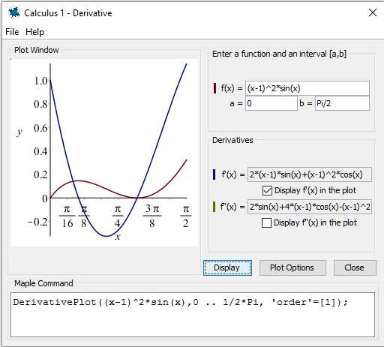
\includegraphics[width=0.8\textwidth]{tutorials/figures/DerivativeTutorQ1-1-eps-converted-to.pdf}
\vspace{-1cm}
\end{figure}
\marginnote[-4cm]{When typing out the function in the tutor, you will not have access to the palettes toolbar in Maple. You will need to type out commands such as \texttt{sqrt()} for square roots. You must also include the symbol * for multiplication.}

\begin{figure}[h]
\caption{You can optionally specify the axes ranges as well as $1:1$ scaling.}
\centering
\adjincludegraphics[width=\textwidth,trim={{0.2\width} 0 0 0},clip]{tutorials/figures/DerivativeTutorQ1-2-eps-converted-to.pdf}
\end{figure}

\section{The Differentiation Methods Tutor}

The Differentiation Methods tutor is useful for showing each individual differentiation rule as a separate step when finding the derivative of a given function.

\begin{figure}[h]
\caption{Opening up the Differentiation Methods tutor using menus.}
\centering
\adjincludegraphics[width=\textwidth]{tutorials/figures/DiffTutorLoad1-eps-converted-to.pdf}
\end{figure}

\begin{figure}[h]
\caption{Opening up the Differentiation Methods tutor using commands. The \texttt{Student[Calculus1]} package is required.}
\centering
\adjincludegraphics[width=\textwidth]{tutorials/figures/DiffTutorLoad2-eps-converted-to.pdf}
\end{figure}

\clearpage

\subsection{Differentiating $x^2\cos(x)$ using Product and Power Rules}

\begin{figure}[h]
\caption{Using the Get Hint button gives you suggestions as to what differentiation rule to use.}
\centering
\adjincludegraphics[width=0.8\textwidth,trim={0 {0.6\height} 0 0},clip]{tutorials/figures/DiffTutorQ1-1-eps-converted-to.pdf}
\adjincludegraphics[width=0.8\textwidth,trim={0 {0.3\height} 0 0},clip]{tutorials/figures/DiffTutorQ1-2-eps-converted-to.pdf}
\end{figure}

\marginnote[-4cm]{When typing out the function in the tutor, you will not have access to the palettes toolbar in Maple. You will need to type out commands such as \texttt{sqrt()} for square roots. You must also include the symbol * for multiplication.}

\begin{figure}[h]
\caption{If a rule cannot be applied, then the tutor will provide additional hints.}
\centering
\adjincludegraphics[width=0.8\textwidth,trim={0 {0.28\height} 0 0},clip]{tutorials/figures/DiffTutorQ1-3-eps-converted-to.pdf}
\end{figure}

\clearpage

\begin{figure}[h]
\caption{Using the product rule, the power rule, and the derivative of $\cos(x)$ to differentiate $x^2\cos(x)$.}
\centering
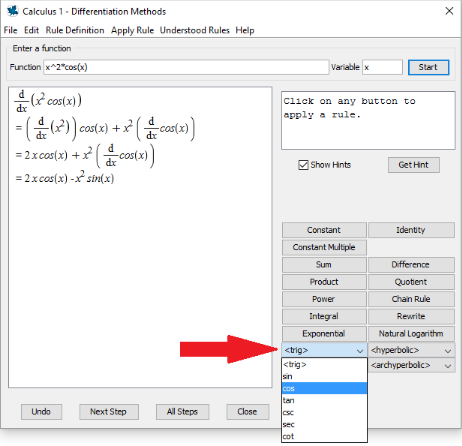
\includegraphics[width=0.8\textwidth]{tutorials/figures/DiffTutorQ1-4-eps-converted-to.pdf}\\
\end{figure}

\subsection{Differentiating $\frac{\sin(x)}{x\tan(x)}$ using Rewrite and Quotient Rule}

\begin{figure}[h]
\caption{Using the Rewrite button allows you to replace an expression with another equivalent expression.}
\centering
\adjincludegraphics[width=0.8\textwidth,trim={0 {0.2\height} 0 0},clip]{tutorials/figures/DiffTutorQ2-1-eps-converted-to.pdf}
%\adjincludegraphics[width=0.8\textwidth,trim={0 {0.7\height} 0 0},clip]{tutorials/figures/DiffTutorQ2-2-eps-converted-to.pdf}
\end{figure}

\clearpage

\begin{figure}[h]
\caption{Applying the quotient rule to differentiate $\frac{\sin(x)}{x\tan(x)}$.}
\centering
\adjincludegraphics[width=0.8\textwidth,trim={0 {0.3\height} 0 0},clip]{tutorials/figures/DiffTutorQ2-3-eps-converted-to.pdf}
\end{figure}

\section{Newton's Method} \label{sec:newtonsmethod}

Suppose we start with the function $f(x) = {\rm e}^x - 2$. We know that the root of this function is $x = \ln 2$. If we wish to evaluate $\ln 2$ as a decimal, we can simply use \texttt{fsolve()}.

\index{mathematical functions!exponential}
\index{solving equations!fsolve}

\index{packages!Student[Calculus1]}

\begin{maplegroup}
\begin{mapleinput}
\mapleinline{active}{1d}{f(x) := exp(x) - 2;
}{}
\end{mapleinput}
\mapleresult
\begin{maplelatex}
\mapleinline{inert}{2d}{f := proc (x) options operator, arrow; exp(x)-2 end proc}{\[\displaystyle f\, := \,x\mapsto {{\rm e}^{x}}-2\]}
\end{maplelatex}
\end{maplegroup}

\begin{maplegroup}
\begin{mapleinput}
\mapleinline{active}{1d}{fsolve(f(x) = 0);
}{}
\end{mapleinput}
\mapleresult
\begin{maplelatex}
\mapleinline{inert}{2d}{.6931471806}{\[\displaystyle  0.6931471806\]}
\end{maplelatex}
\end{maplegroup}

We can also find this root by applying Newton's method with an initial guess of $x=2$. We need to load the \texttt{Student[Calculus1]} package before we use the \texttt{NewtonsMethod()} command. 

Optional parameters may be included to change how the result is displayed and how many iterations of the method are performed.

\index{Newton's method!NewtonsMethod!output options}
\index{Newton's method!NewtonsMethod!iterations}

\begin{table}
\label{tbl:newtonsmethod_options}
\centering
\begin{tabular}{lp{2.5in}}
\hline
Parameter & Description\\
\hline
\texttt{output = value}			& Outputs the numerical result of Newton's method.\\
\texttt{output = plot}			& Outputs a plot showing the tangent line approximation approach to finding the root.\\
\texttt{output = animation}		& Much like the \texttt{plot} output, only with each iteration as a separate frame.\\
\texttt{output = sequence}		& Outputs the original guess and the result of each iteration of Newton's method.\\
\texttt{iterations = }$n$		& Specifies the number of iterations to perform in Newton's method.\\
\hline
\end{tabular}
\caption{A list of optional parameters for the \texttt{NewtonsMethod()} command.}
\end{table}

\clearpage

\begin{maplegroup}
\begin{mapleinput}
\mapleinline{active}{1d}{with(Student[Calculus1]):
}{}
\end{mapleinput}
\end{maplegroup}

\index{packages!with}
\index{packages!Student[Calculus1]}

\begin{maplegroup}
\begin{mapleinput}
\mapleinline{active}{1d}{NewtonsMethod(f(x), x=2, output=plot);
}{}
\end{mapleinput}
\mapleresult
\mapleplot{tutorials/figures/newtonsmethodplot2d1-eps-converted-to.pdf}
\end{maplegroup}

If we wish to simply evaluate the root, the \texttt{output=plot} option may be omitted. For more accuracy, the algorithm can be run with additional iterations.

\index{Newton's method!NewtonsMethod}

\begin{maplegroup}
\begin{mapleinput}
\mapleinline{active}{1d}{NewtonsMethod(f(x), x=2);
}{}
\end{mapleinput}
\mapleresult
\begin{maplelatex}
\mapleinline{inert}{2d}{.6931471814}{\[\displaystyle  0.6931471814\]}
\end{maplelatex}
\end{maplegroup}

\index{Newton's method!NewtonsMethod!output options}
\index{Newton's method!NewtonsMethod!iterations}

\marginnote[1cm]{The default number of iterations for \texttt{NewtonsMethod()} with the parameter \texttt{ouput=sequence} is $5$.}
\begin{maplegroup}
\begin{mapleinput}
\mapleinline{active}{1d}{NewtonsMethod(f(x), x=2, output=sequence);
}{}
\end{mapleinput}
\mapleresult
\begin{maplelatex}
\mapleinline{inert}{2d}{2, 1.270670566, .8319573035, .7023505839, .6931894021, .6931471814}{\[\displaystyle \begin{array}{l}2,\, 1.270670566,\, 0.8319573035,\, 0.7023505839,\, \\ 0.6931894021,\, 0.6931471814 \end{array}\]}
\end{maplelatex}
\end{maplegroup}

\begin{maplegroup}
\begin{mapleinput}
\mapleinline{active}{1d}{NewtonsMethod(f(x), x=2, iterations=10);
}{}
\end{mapleinput}
\mapleresult
\begin{maplelatex}
\mapleinline{inert}{2d}{.6931471804}{\[\displaystyle  0.6931471804\]}
\end{maplelatex}
\end{maplegroup}

\begin{maplegroup}
\begin{mapleinput}
\mapleinline{active}{1d}{}{}
\end{mapleinput}
\end{maplegroup}